\documentclass[a4paper,titlepage]{article}
\usepackage[utf8]{inputenc}
\usepackage{fullpage}
\usepackage{indentfirst}
\usepackage[per-mode=symbol]{siunitx}
\usepackage{listings}
\usepackage{graphicx}
\usepackage{color}
\usepackage{amsmath}
\usepackage{array}
\usepackage[hidelinks]{hyperref}
\usepackage[format=plain,font=it]{caption}
\usepackage{subcaption}
\usepackage{standalone}
\usepackage[nottoc]{tocbibind}
\usepackage[noabbrev,capitalize,nameinlink]{cleveref}
\usepackage{listings}
\usepackage{xspace}
\usepackage{tikz}
\usepackage{circuitikz}
\usepackage{titlesec}
\usepackage[cache=false]{minted}
\usepackage{booktabs}
\usepackage{csvsimple}
\newcommand{\MATLAB}{\textsc{Matlab}\xspace}
\usepackage{siunitx}
\usepackage[super]{nth}
\usepackage[titletoc]{appendix}

% Custom commands
\newcommand\numberthis{\addtocounter{equation}{1}\tag{\theequation}}
\newcommand{\code}[1]{\texttt{#1}}
\newcolumntype{P}[1]{>{\centering\arraybackslash}p{#1}}

\setminted{linenos,breaklines,fontsize=auto}

%\titleformat*{\section}{\normalsize\bfseries}
%\titleformat*{\subsection}{\small\bfseries}
\renewcommand{\thesubsection}{\thesection.\alph{subsection}}
\providecommand*{\listingautorefname}{Listing}
\newcommand*{\Appendixautorefname}{Appendix}


\begin{document}
	\sloppy	
	
	\begin{center}
		{\LARGE \bf ECSE 597: Circuit Simulations and Modeling}\\
		{\large Assignment 4, \quad \today}\\
		{\large Wenjie Wei, 260685967}
	\end{center}

	\section{Results of Circuit Simulation}
		Figure \ref{res} shows the result curve of the testing circuit. The results of the three testing points: -10V, -2V, and 8V are indicated in the plot:
		\begin{itemize}
			\item $V_i = -10V, \quad V_o = -3.43V$;
			\item $V_i = -1.92V, \quad V_o = -1.92V$;
			\item $V_i = 3.28V, \quad V_o = -7.98V$;
		\end{itemize}
		
		Because of the nature of the \MATLAB function \texttt{\textbf{linspace()}}, only the results at the nearest points are shown. 
		\begin{figure}[H]
			\centering
			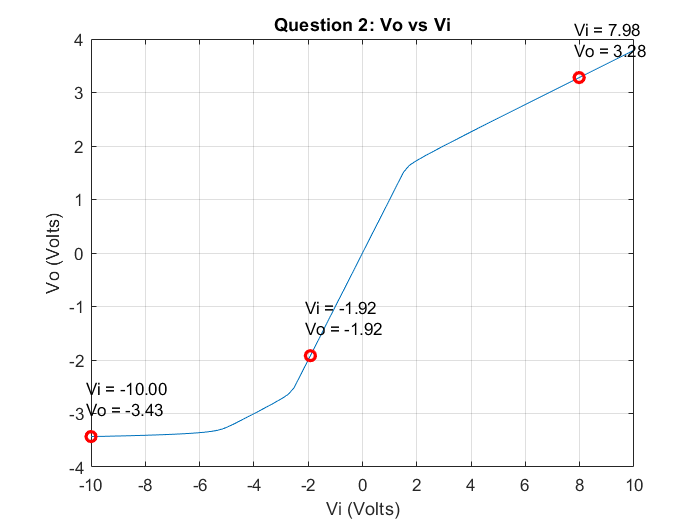
\includegraphics[width=0.7\linewidth]{graph}
			\caption{Results of the Test Circuit Indicating Three Test Points}
			\label{res}
		\end{figure}
	\newpage
	
	\begin{appendices}		
		\section{Code Listings} \label{appendix:code}
		
			\setminted{linenos,breaklines,fontsize=\footnotesize}
			
			\begin{center}
				\captionof{listing}{MATLAB Function to Compute the DC Solution (\texttt{dcsolvealpha.m}).}
				\inputminted{matlab}{../../src/a4/dcsolvealpha.m}
				\label{dcsolve}
			\end{center}
			\begin{center}
				\captionof{listing}{MATLAB Function to Compute the DC Solution Using Power Ramping (\texttt{dcsolvecont.m}).}
				\inputminted{matlab}{../../src/a4/dcsolvecont.m}
				\label{dcsolvecont}
			\end{center}
	\end{appendices}
\end{document}